\documentclass[aspectratio=169]{beamer}

\usetheme{Madrid}
\usepackage{todonotes}
\usepackage{graphicx}
\usepackage{xcolor}
\usepackage{subfig}
%%\usepackage[noend]{algpseudocode}


%\usepackage{algorithm}
%\usepackage{algorithmic}
\usepackage{algorithm,algpseudocode}

\usepackage{blkarray}
\usepackage{amsmath}
\usepackage{xspace}
\usepackage{float}
\usepackage{appendixnumberbeamer}


\usepackage{booktabs}

%\usepackage{enumitem}


\usepackage{tikz}
\usetikzlibrary{matrix, decorations, patterns, positioning, shapes, 3d,calc, intersections, arrows, fit, hobby}


\newcommand{\brown}[1]{{\color{brown} #1 }}

\definecolor{pastelviolet}{rgb}{0.8, 0.6, 0.79}
\definecolor{babyblueeyes}{rgb}{0.63, 0.79, 0.95}
\definecolor{pastelyellow}{rgb}{0.99, 0.99, 0.59}
\definecolor{pastelgreen1}{rgb}{0.47, 0.87, 0.47}
\definecolor{pastelgreen}{rgb}{0, 1, 0}
\definecolor{pastelred}{rgb}{1.0, 0.41, 0.38}
\colorlet{patternblue}{blue!60}


\graphicspath{{./diagrams/}{./Figs/}{./plots/}}

\usetheme{Madrid}


\usepackage{bm}
% matrices
\newcommand{\M}[2][]{{\bm{#1\mathbf{\MakeUppercase{#2}}}}} 

\usepackage{pgfplots}
\usepackage{pgfplotstable}
\usepackage{tikz}
\usepackage{ifthen}
\usetikzlibrary{calc} % Required for coordinate calculations
\pgfplotsset{compat=1.16}

% Define custom colors
\definecolor{color3}{RGB}{70,130,180}   % SteelBlue
\definecolor{color2}{RGB}{220,20,60}    % Crimson
\definecolor{color1}{RGB}{34,139,34}    % ForestGreen
\definecolor{color4}{RGB}{255,165,0}    % Orange
\definecolor{color5}{RGB}{128,128,128}  % Gray
\definecolor{color6}{RGB}{138,43,226}   % BlueViolet
\definecolor{color7}{RGB}{255,105,180}  % HotPink
\definecolor{color8}{RGB}{0,206,209}    % DarkTurquoise
\definecolor{color9}{RGB}{210,105,30}   % Chocolate


% Dummy variables for modes & groups
\newcommand{\algoa}{1Dred}
\newcommand{\algob}{1Dnored}
\newcommand{\gen}{MatMul_Gen}
\newcommand{\comm}{MatMul_Comm}
\newcommand{\impla}{CPP}
\newcommand{\implb}{Python}
\newcommand{\proca}{4}
\newcommand{\procb}{8}
\newcommand{\procc}{16}
\newcommand{\procd}{32}
\newcommand{\proce}{64}
\newcommand{\procf}{128}



% Control flags
\newif\ifylabel \ylabeltrue
\newif\iflegend \legendtrue

% === 1 PLOT OPTIONS ===
\newcommand{\matmulCPUrankFiveH}{
	ybar stacked,
	reverse legend,
	bar width=4pt,
	width=5.2cm, 
	height=4.5cm,
	enlarge x limits=0.05,    % add spacing at left and right edges
	\ifylabel
	ylabel={Time (seconds)}, 
	\fi
	y label style={yshift=-0.2cm},
	ymin=0,
	ymax=0.26,
	symbolic x coords={Algo-\gen-\proca,Algo-\comm-\proca,,Algo-\gen-\procb,Algo-\comm-\procb,,Algo-\gen-\procc,Algo-\comm-\procc,,Algo-\gen-\procd,Algo-\comm-\procd,,Algo-\gen-\proce,Algo-\comm-\proce,,Algo-\gen-\procf,Algo-\comm-\procf},
	xticklabels={Gen,Gen,Gen,Gen,Gen,Gen,Comm,Comm,Comm,Comm,Comm,Comm},  % need to match order in datafile
	xtick=data,
	x tick label style={xshift=0.19cm, rotate=45, anchor=east}, % xshift moves Old/New along x axis
	xlabel={P}, 
	xlabel style={yshift=-0.45cm}, % Moves Algorithm-Mode
	%legend pos={north west},
	legend style={
		at={(0.65,1.1)},     % Position (x,y)
		anchor=west,         % Anchor point of legend box
	},
	legend columns=2,
	legend style={draw=none, cells={align=left}, nodes={scale=0.7}},
}

% === 2 PLOT OPTIONS ===
\newcommand{\matmulCPUrankFiveT}{
	ybar stacked,
	reverse legend,
	bar width=4pt,
	width=5.2cm, height=4.5cm,
	enlarge x limits=0.05,    % add spacing at left and right edges
	\ifylabel
	%ylabel={Time (seconds)}, 
	\fi
	y label style={yshift=-0.2cm},
	ymin=0,
	ymax=.85,
	symbolic x coords={Algo-\gen-\proca,Algo-\comm-\proca,,Algo-\gen-\procb,Algo-\comm-\procb,,Algo-\gen-\procc,Algo-\comm-\procc,,Algo-\gen-\procd,Algo-\comm-\procd,,Algo-\gen-\proce,Algo-\comm-\proce,,Algo-\gen-\procf,Algo-\comm-\procf},
	xticklabels={Gen,Gen,Gen,Gen,Gen,Gen,Comm,Comm,Comm,Comm,Comm,Comm},  % need to match order in datafile
	xtick=data,
	x tick label style={xshift=0.19cm, rotate=45, anchor=east}, % xshift moves Old/New along x axis
	xlabel={P}, 
	xlabel style={yshift=-0.45cm}, % Moves Algorithm-Mode
	legend pos={north west},
	legend columns=2,
	legend style={draw=none, cells={align=left}, nodes={scale=0.7}},
}

%% === 3 PLOT OPTIONS ===
%\newcommand{\matmulGPUrankFiveH}{
%	ybar stacked,
%	reverse legend,
%	bar width=4pt,
%	width=5.2cm, height=4.5cm,
%	enlarge x limits=0.05,    % add spacing at left and right edges
%	\ifylabel
%	ylabel={Time (seconds)}, 
%	\fi
%	y label style={yshift=-0.2cm},
%	ymin=0,
%	ymax=0.3,
%	symbolic x coords={Algo-\gen-\proca,Algo-\comm-\proca,,Algo-\gen-\procb,Algo-\comm-\procb,,Algo-\gen-\procc,Algo-\comm-\procc,,Algo-\gen-\procd,Algo-\comm-\procd,,Algo-\gen-\proce,Algo-\comm-\proce,,Algo-\gen-\procf,Algo-\comm-\procf},
%	xticklabels={Gen,Gen,Gen,Gen,Gen,Gen,Comm,Comm,Comm,Comm,Comm,Comm},  % need to match order in datafile
%	xtick=data,
%	x tick label style={xshift=0.19cm, rotate=45, anchor=east}, % xshift moves Old/New along x axis
%	xlabel={P}, 
%	xlabel style={yshift=-0.45cm}, % Moves Algorithm-Mode
%	%legend pos={north west},
%	legend style={
%		at={(0.65,1.1)},     % Position (x,y)
%		anchor=west,         % Anchor point of legend box
%	},
%	legend columns=2,
%	legend style={draw=none, cells={align=left}, nodes={scale=0.7}},
%}
%
%% === 4 PLOT OPTIONS ===
%\newcommand{\matmulGPUrankFiveT}{
%	ybar stacked,
%	reverse legend,
%	bar width=4pt,
%	width=5.2cm, height=4.5cm,
%	enlarge x limits=0.05,    % add spacing at left and right edges
%	\ifylabel
%	%ylabel={Time (seconds)}, 
%	\fi
%	y label style={yshift=-0.2cm},
%	ymin=0,
%	ymax=0.4,
%	symbolic x coords={Algo-\gen-\proca,Algo-\comm-\proca,,Algo-\gen-\procb,Algo-\comm-\procb,,Algo-\gen-\procc,Algo-\comm-\procc,,Algo-\gen-\procd,Algo-\comm-\procd,,Algo-\gen-\proce,Algo-\comm-\proce,,Algo-\gen-\procf,Algo-\comm-\procf},
%	xticklabels={Gen,Gen,Gen,Gen,Gen,Gen,Comm,Comm,Comm,Comm,Comm,Comm},  % need to match order in datafile
%	xtick=data,
%	x tick label style={xshift=0.19cm, rotate=45, anchor=east}, % xshift moves Old/New along x axis
%	xlabel={P}, 
%	xlabel style={yshift=-0.45cm}, % Moves Algorithm-Mode
%	legend pos={north west},
%	legend columns=2,
%	legend style={draw=none, cells={align=left}, nodes={scale=0.7}},
%}

% === 5 PLOT OPTIONS ===
\newcommand{\nystromCPUrankFiveH}{
	ybar stacked,
	reverse legend,
	bar width=4pt,
	width=5.2cm, height=4.5cm,
	enlarge x limits=0.05,    % add spacing at left and right edges
	\ifylabel
	ylabel={Time (seconds)}, 
	\fi
	y label style={yshift=-0.2cm},
	ymin=0,
	ymax=0.035,
	symbolic x coords={Algo-\algoa-\proca,Algo-\algob-\proca,,Algo-\algoa-\procb,Algo-\algob-\procb,,Algo-\algoa-\procc,Algo-\algob-\procc,,Algo-\algoa-\procd,Algo-\algob-\procd,,Algo-\algoa-\proce,Algo-\algob-\proce,,Algo-\algoa-\procf,Algo-\algob-\procf},
	xticklabels={Redist,Redist,Redist,Redist,Redist,Redist,No-Redist,No-Redist,No-Redist,No-Redist,No-Redist,No-Redist},  % need to match order in datafile
	xtick=data,
	x tick label style={xshift=0.1cm, rotate=65, anchor=east}, % xshift moves Old/New along x axis
	xlabel={P}, 
	xlabel style={yshift=-0.15cm}, % Moves Algorithm-Mode
	%legend pos={north east},
	legend style={
		at={(0.55,1.1)},     % Position (x,y)
		anchor=west,         % Anchor point of legend box
	},
	legend columns=3,
	legend style={draw=none, cells={align=left}, nodes={scale=0.7}},
}

% === 6 PLOT OPTIONS ===
\newcommand{\nystromCPUrankFiveT}{
	ybar stacked,
	reverse legend,
	bar width=4pt,
	width=5.2cm, height=4.5cm,
	enlarge x limits=0.05,    % add spacing at left and right edges
	\ifylabel
	%ylabel={Time (seconds)}, 
	\fi
	y label style={yshift=-0.2cm},
	ymin=0,
	ymax=0.2,
	symbolic x coords={Algo-\algoa-\proca,Algo-\algob-\proca,,Algo-\algoa-\procb,Algo-\algob-\procb,,Algo-\algoa-\procc,Algo-\algob-\procc,,Algo-\algoa-\procd,Algo-\algob-\procd,,Algo-\algoa-\proce,Algo-\algob-\proce,,Algo-\algoa-\procf,Algo-\algob-\procf},
	xticklabels={Redist,Redist,Redist,Redist,Redist,Redist,No-Redist,No-Redist,No-Redist,No-Redist,No-Redist,No-Redist},  % need to match order in datafile
	xtick=data,
	x tick label style={xshift=0.1cm, rotate=65, anchor=east}, % xshift moves Old/New along x axis
	xlabel={P}, 
	xlabel style={yshift=-0.15cm}, % Moves Algorithm-Mode
	legend pos={north east},
	% legend columns=2,
	legend style={draw=none, cells={align=left}, nodes={scale=0.7}},
}

% === 7 PLOT OPTIONS ===
\newcommand{\nystromGPUrankFiveH}{
	ybar stacked,
	reverse legend,
	bar width=4pt,
	width=5.2cm, height=4.5cm,
	enlarge x limits=0.05,    % add spacing at left and right edges
	\ifylabel
	ylabel={Time (seconds)}, 
	\fi
	y label style={yshift=-0.2cm},
	ymin=0,
	ymax=0.15,
	symbolic x coords={Algo-\algoa-\proca,Algo-\algob-\proca,,Algo-\algoa-\procb,Algo-\algob-\procb,,Algo-\algoa-\procc,Algo-\algob-\procc,,Algo-\algoa-\procd,Algo-\algob-\procd,,Algo-\algoa-\proce,Algo-\algob-\proce,,Algo-\algoa-\procf,Algo-\algob-\procf},
	xticklabels={Redist,Redist,Redist,Redist,Redist,Redist,No-Redist,No-Redist,No-Redist,No-Redist,No-Redist,No-Redist},  % need to match order in datafile
	xtick=data,
	x tick label style={xshift=0.1cm, rotate=65, anchor=east}, % xshift moves Old/New along x axis
	xlabel={P}, 
	xlabel style={yshift=-0.45cm}, 
	%legend pos={north west},
	legend style={
		at={(0.45,1.1)},     % Position (x,y)
		anchor=west,         % Anchor point of legend box
	},
	legend columns=3,
	legend style={draw=none, cells={align=left}, nodes={scale=0.7}},
}

% === 8 PLOT OPTIONS ===
\newcommand{\nystromGPUrankFiveT}{
	ybar stacked,
	reverse legend,
	bar width=4pt,
	width=5.2cm, height=4.5cm,
	enlarge x limits=0.05,    % add spacing at left and right edges
	\ifylabel
	%ylabel={Time (seconds)}, 
	\fi
	y label style={yshift=-0.2cm},
	ymin=0,
	ymax=0.3,
	symbolic x coords={Algo-\algoa-\proca,Algo-\algob-\proca,,Algo-\algoa-\procb,Algo-\algob-\procb,,Algo-\algoa-\procc,Algo-\algob-\procc,,Algo-\algoa-\procd,Algo-\algob-\procd,,Algo-\algoa-\proce,Algo-\algob-\proce,,Algo-\algoa-\procf,Algo-\algob-\procf},
	xticklabels={Redist,Redist,Redist,Redist,Redist,Redist,No-Redist,No-Redist,No-Redist,No-Redist,No-Redist,No-Redist},  % need to match order in datafile
	xtick=data,
	x tick label style={xshift=0.1cm, rotate=65, anchor=east}, % xshift moves Old/New along x axis
	xlabel={P}, 
	xlabel style={yshift=-0.45cm}, 
	legend pos={north west},
	legend columns=1,
	legend style={draw=none, cells={align=left}, nodes={scale=0.7}},
}

% === 9 PLOT OPTIONS ===
\newcommand{\cppVSpython}{
	ybar stacked,
	reverse legend,
	bar width=7pt,
	width=8.4cm, height=6.5cm,
	enlarge x limits=0.05,    % add spacing at left and right edges
	\ifylabel
	ylabel={Time (seconds)}, 
	\fi
	y label style={yshift=-0.2cm},
	ymin=0,
	ymax=180,
	symbolic x coords={Algo-\impla-\proca,Algo-\implb-\proca,,Algo-\impla-\procb,Algo-\implb-\procb,,Algo-\impla-\procc,Algo-\implb-\procc,,Algo-\impla-\procd,Algo-\implb-\procd,,Algo-\impla-\proce,Algo-\implb-\proce,,Algo-\impla-\procf,Algo-\implb-\procf},
	xticklabels={CPP,CPP,CPP,CPP,CPP,CPP,Python,Python,Python,Python,Python,Python},  % need to match order in datafile
	xtick=data,
	x tick label style={xshift=0.19cm, rotate=45, anchor=east}, % xshift moves Old/New along x axis
	xlabel={P}, 
	xlabel style={yshift=-0.45cm}, % Moves Algorithm-Mode
	legend pos={north east},
	legend columns=2,
	legend style={draw=none, cells={align=left}, nodes={scale=0.7}},
}

% === 10 PLOT OPTIONS ===
\newcommand{\nystromCPUrankFiveTall}{
	ybar stacked,
	reverse legend,
	bar width=4pt,
	width=5.2cm, height=5.5cm,
	enlarge x limits=0.05,    % add spacing at left and right edges
	\ifylabel
	ylabel={Time (seconds)}, 
	\fi
	y label style={yshift=-0.2cm},
	ymin=0,
	ymax=21.0,
	symbolic x coords={Algo-\algoa-\proca,Algo-\algob-\proca,,Algo-\algoa-\procb,Algo-\algob-\procb,,Algo-\algoa-\procc,Algo-\algob-\procc,,Algo-\algoa-\procd,Algo-\algob-\procd,,Algo-\algoa-\proce,Algo-\algob-\proce,,Algo-\algoa-\procf,Algo-\algob-\procf},
	xticklabels={Redist,Redist,Redist,Redist,Redist,Redist,No-Redist,No-Redist,No-Redist,No-Redist,No-Redist,No-Redist},  % need to match order in datafile
	xtick=data,
	x tick label style={xshift=0.1cm, rotate=65, anchor=east}, % xshift moves Old/New along x axis
	xlabel={P}, 
	xlabel style={yshift=-0.15cm}, % Moves Algorithm-Mode
	legend style={
		at={(-0.18,1.1)},     % Position (x,y)
		anchor=west,         % Anchor point of legend box
	},
	legend columns=6,
	legend style={draw=none, cells={align=left}, nodes={scale=0.7}},
}

% === 11 PLOT OPTIONS ===
\newcommand{\nystromGPUrankFiveTall}{
	ybar stacked,
	reverse legend,
	bar width=4pt,
	width=5.2cm, height=5.5cm,
	enlarge x limits=0.05,    % add spacing at left and right edges
	\ifylabel
	%ylabel={Time (seconds)}, 
	\fi
	y label style={yshift=-0.2cm},
	ymin=0,
	ymax=1.3,
	symbolic x coords={Algo-\algoa-\proca,Algo-\algob-\proca,,Algo-\algoa-\procb,Algo-\algob-\procb,,Algo-\algoa-\procc,Algo-\algob-\procc,,Algo-\algoa-\procd,Algo-\algob-\procd,,Algo-\algoa-\proce,Algo-\algob-\proce,,Algo-\algoa-\procf,Algo-\algob-\procf},
	xticklabels={Redist,Redist,Redist,Redist,Redist,Redist,No-Redist,No-Redist,No-Redist,No-Redist,No-Redist,No-Redist},  % need to match order in datafile
	xtick=data,
	x tick label style={xshift=0.1cm, rotate=65, anchor=east}, % xshift moves Old/New along x axis
	xlabel={P}, 
	xlabel style={yshift=-0.15cm}, % Moves Algorithm-Mode
	legend style={
		at={(0.05,1.1)},     % Position (x,y)
		anchor=west,         % Anchor point of legend box
	},
	legend columns=5,
	legend style={draw=none, cells={align=left}, nodes={scale=0.7}},
}
%************************************************************************


\begin{document}

%\title[Communication costs with random matrices]{Nyström Low-Rank Approximation: Communication Lower Bounds and Algorithms} % The short title appears at the bottom of every slide, the full title is only on the title page
\title[Communication costs with random matrices]{Parallel Communication Lower Bounds and Algorithms for Computations with Random Matrices} % The short title appears at the bottom of every slide, the full title is only on the title page


%%\author{John Smith} % Your name
%%\institute[UCLA] % Your institution as it will appear on the bottom of every slide, may be shorthand to save space
%%{
%%University of California \\ % Your institution for the title page
%%\medskip
%%\textit{john@smith.com} % Your email address
%%}

\author[Suraj {\sc Kumar}]{\small Hussam {\sc Al Daas}\inst{1}, Grey {\sc Ballard}\inst{2}, Laura {\sc Grigori}\inst{3}, Md Taufique {\sc Hussain}\inst{2}, \underline{Suraj {\sc Kumar}}\inst{4}, Md Marufur {\sc Rahman}\inst{2} and Kathryn {\sc Rouse}\inst{5}\vspace*{-0.15cm}}
\institute[Inria Lyon]{\inst{1} Rutherford Appleton Laboratory, UK \and %
	\inst{2} Wake Forest University, USA \and
	\inst{3} Ecole Polytechnique Fédérale de Lausanne (EPFL), Switzerland \and
	\inst{4} Inria Lyon, France \and
	\inst{5} Inmar Intelligence, USA}
\date[METT XI (2026)]{11th Workshop on Matrix Equations and Tensor Techniques (Jan 08, 2026)} % Date, can be changed to a custom date




\begin{frame}
	\titlepage % Print the title page as the first slide
\end{frame}

%\begin{frame}{Table of Contents} 
%	\tableofcontents[currentsection] % Output the table of contents (all sections on one slide)
%\end{frame}

\begin{frame}{Communication lower bounds for a computation on $P$ processors}
	minimum amount of communication required to perform the computation in parallel
	\vfill
	
%	\begin{itemize}
%		\item Lower bounds: minimum amount of communication required to perform the computation in parallel
%		\vfill
%	\end{itemize}
	\begin{block}{Should avoid such settings}
		\begin{itemize}
			\item If all operations are performed on a single processor, then no communication is required
			\item If data is duplicated on all processors, then communication may not be necessary 
		\end{itemize}
	\end{block}
	\vfill
	\begin{block}{Our assumptions}
		\begin{itemize}
			\item Load balanced computation: each processor performs equal amount of operations
			\vfill
			\item There is one copy of data in the system
		\end{itemize}
	\end{block}
	\vfill
	
	\begin{itemize}
		\item There exist one processor that has at most $1/P$th amount of overall data -- we examine the required data transfers for this processor to establish the lower bound
%		\item We consider communication cost along the critical path of the algorithm -- the path along which the sum of all data transfers is maximum
	\end{itemize}

\end{frame}
\begin{frame}{Communication costs}
	\begin{itemize}
		\item Communication cost: latency cost (number of messages) and bandwidth cost (volume of data transfers)
		\vfill
		\item Focus on bandwidth costs -- it dominates when messages are large
		\vfill
	\end{itemize}
\vfill
\begin{block}{Communication cost of an algorithm}
	\begin{itemize}
		\item Cost along the critical path -- the path along which the communication (bandwidth) cost is maximum
	\end{itemize}
\end{block}
\vfill
\end{frame}

\begin{frame}{Focus on $A\Omega$ and $\Omega^T A\Omega$ computations}
	\begin{block}{$B=A\Omega$ computation}
		\begin{itemize}
			\item $A \in \mathbb{R}^{n_1\times n_2}$ and $\Omega$ is a $n_2 \times r$ random matrix
			\vfill
			\item Fundamental to all randomized linear algebra techniques including randomized SVD 
		\end{itemize}
	\end{block}
	\vfill
	\begin{block}{$B=A\Omega$ and $C=\Omega^T A\Omega$ computations together}
		\begin{itemize}
			%			\item 
			\item $A$ is a $n\times n$ matrix and $\Omega$ is a $n \times r$ random matrix
			\item Useful for Nystrom approximation, $\widetilde{\M{A}} = (\M{A}\M{\Omega}) (\M{\Omega}^T\M{A}\M{\Omega})^\dag (\M{A}\M{\Omega})^T$
		\end{itemize}
	\end{block}
	\vfill
	$r$ is (much) less than the contracted dimension ($r\leq n_2$ and $r\leq n$).
\end{frame}


\section{Existing results for classical matrix multiplication}
\begin{frame}{Table of Contents} 
	\tableofcontents[hideallsubsections] % Output the table of contents (all sections on one slide)
\end{frame}
\begin{frame}{Table of Contents} 
	\tableofcontents[currentsection, hideallsubsections] % Output the table of contents (all sections on one slide)
\end{frame}
\begin{frame}{Classical matrix multiplication bound}
	\begin{itemize}
		\item $C=AB$ with $A \in \mathbb{R}^{n_1\times n_2}, B \in \mathbb{R}^{n_2\times n_3}$, and $C \in \mathbb{R}^{n_1\times n_3}$
	\end{itemize}
\vfill
Let $k=\min(n_1,n_2,n_3) \leq \ell= median(n_1,n_2,n_3) \leq m=\max(n_1,n_2,n_3)$.
\vfill
\begin{itemize}
	\item $\phi_A, \phi_B, \phi_C$: number of elements accessed by a processor in arrays $A$, $B$, $C$
	\vfill
	\item Minimum number of elements accessed in the critical path = $\phi_A + \phi_B + \phi_C$
	\vfill
%\end{itemize}
\begin{center}
	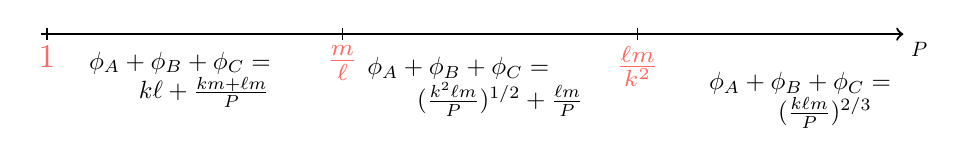
\begin{tikzpicture}[scale=0.75, every node/.style={transform shape}]
	%%\draw (-2,0) -- node[below] {a} ++(2,0) -- node[above] {b} ++(2,0);
	%%\draw (-0.1,0) -- ++(5,0) -- ++(5,0);
	\draw [->, thick] (-0.1,0) -- (14.5,0) node [below right] {$P$};
	\draw (0, 0.1) -- node [below, pastelred, scale=1.6]{$1$}(0,-0.1);
	\draw (5, 0.1) -- node [below, pastelred, scale=1.6]{$\frac{m}{\ell}$}(5,-0.1);
	\draw (10, 0.1) -- node [below, pastelred, scale=1.6] {$\frac{\ell m}{k^2}$}(10,-0.1);
	
	\node[align=left,below,scale=1.2] at (2.25, -0.15) {$\phi_A + \phi_B + \phi_C =$ \\ $\qquad  k\ell + \frac{km + \ell m}{P}$};
	\node[align=left,below,scale=1.2] at (7.25, -0.25) {$\phi_A + \phi_B + \phi_C =$ \\ $\qquad (\frac{k^2\ell m}{P})^{1/2} + \frac{\ell m}{P}$};
	\node[align=center,below,scale=1.2] at (12.75, -0.5) {$\phi_A + \phi_B + \phi_C =$ \\ $\qquad  (\frac{k\ell m}{P})^{2/3}$};	
	\end{tikzpicture}
\end{center}
%\begin{itemize}
	\item Communication lower bound = $\phi_A + \phi_B + \phi_C - \frac{n_1n_2+n_2n_3+n_1n_3}{P}$
\end{itemize}
\vfill
\centering\brown{Can we improve this bound when one matrix is randomly generated?}
\end{frame}




\section{$A\Omega$ computation}
\subsection{Communication lower bounds}
\begin{frame}{Table of Contents} 
	\tableofcontents[currentsubsection] % Output the table of contents (all sections on one slide)
%	hideothersubsections
\end{frame}

\begin{frame}{Approach to obtain communication lower bounds}
	\begin{minipage}{0.7\linewidth}
		A special case of H\"{o}lder-Brascamp-Lieb (HBL) inequality:
		\begin{itemize}
			\item For the $3$d object $B$, $\phi_{i}\phi_{jk} \ge Volume(B)$
			\item $\phi_{j}$, $\phi_{ik}$: projections of $B$ on $j$-axis and $i-k$ plane
			\item Also implies that: $\phi_{ij}\phi_{ik} \ge Volume(B)$ and $\phi_{jk}\phi_{ik} \ge Volume(B)$
		\end{itemize}
	\end{minipage}$\quad$
	\begin{minipage}{0.25\linewidth}
		\begin{center}
			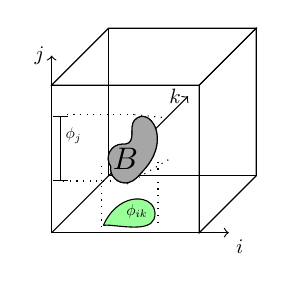
\begin{tikzpicture}[scale=0.375, every node/.style={transform shape}]
			\draw (0,0) -- ++(5,0) -- ++(0, 5) -- ++(-5,0) -- cycle;
			\draw (0,5,0) -- ++(0,0, -5) -- ++(5,0,0) -- ++(0,0,5) -- cycle;
			\draw (5,0,0) -- ++(0,0,-5) -- ++(0,5,0) -- ++(0,0,5) -- cycle;
			\draw (0,0,-5) -- ++(5,0,0) -- ++(0,5,0) -- ++(-5,0,0) -- cycle;
			\draw [<->] (0,6) -- (0,0) -- (6,0);
			\draw [->] (0,0,0) -- (0,0,-12);
			\node [left, scale=2, rotate=0] at (0,0,-12) {$k$};
			\node [below right, scale=2] at (6,0) {$i$};
			\node [left, scale=2] at (0,6) {$j$};
			
			\draw [fill=gray!70] (2,2.25) to [curve through={(2.4,3) .. (2.5,3) .. (2.8,3.8) .. (3.1,2.1) .. (2.6,1.7)}] (2,2.25);
			
%			\node [scale=2] at (2.5,2.5) {$A$};
			\draw [dotted] (1.7,2.25) -- (1.7,0.2);
			\draw [dotted] (3.6,2.4) -- (3.6,0.3);
			
			\draw [fill=green!40] (1.75,0.25) to [curve through={(1.8, 0.35) .. (3.5, 0.65) .. (2,0.25)}] (1.75,0.25);
			\node[above, scale=1.5] at (2.6,0,-0.75) {$\phi_{ik}$};
			
			\draw [dotted] (2,1.75) -- (0.3,1.75);
			\draw [dotted] (2.8,4) -- (0.385,4);
			
			\draw [fill=red!40, |-|] (0.3, 1.75)-- (0.3,3.95);
			 to [curve through={(0.3,1.85) .. (0.3,3.95) }] (0.3,1.75);
%			\draw [fill=red!40] (0.3, 1.75) to [curve through={(0.5,2) .. (1, 2.5) .. (1,3.95) .. (0.2, 2.5)}] (0.3,1.75);
			\node[right, scale=1.5] at (0,3, -0.75) {$\phi_{j}$};
			
%			\draw [fill=yellow!40] (3.85,3.9) to [curve through={(3.7,3.8) .. (3.5,3.4) .. (3.45,3.2)}] (3.85, 3.9);
%			\node [scale=1.5] at (3.65,3.1,-1) {$\phi_{xy}$};
			\draw [dotted] (2.8,4) -- (3.8,3.9);
			\draw [dotted] (2.56,1.65) -- (4,2.5);
			
			\draw [fill=gray!70] (2,2.25) to [curve through={(2.4,3) .. (2.5,3) .. (2.8,3.8) .. (3.1,2.1) .. (2.6,1.7)}] (2,2.25);
			
			\node [scale=3] at (2.5,2.5) {$B$};
			\end{tikzpicture}
		\end{center}
	\end{minipage}
%\vspace*{-0.15cm}
\begin{block}{Constraints for load balanced computation}
	\begin{itemize}
		\item $B=A\Omega$ with $A \in \mathbb{R}^{n_1\times n_2}, B \in \mathbb{R}^{n_1\times r}$, and $\Omega$ is a random matrix
%	\end{itemize}

	\begin{center}
	\vspace*{-0.75cm}
	\begin{align*}
	&\text{for $i = 1{:}n_1$, for $k = 1{:}n_2$, for $j = 1{:}r$}\\
	&\quad \quad C[i][j] += A[i][k]*B[k][j]
	\end{align*}
	\end{center}
	\vspace*{-0.35cm}
%	\begin{itemize}
		\item $\phi_A, \phi_B$ : projections of computations on arrays $A$, $B$
		\item From the HBL inequality: $\phi_A \phi_B \ge \text{number of multiplications per processor}=\frac{n_1n_2r}{P}$
		\item Extra constraints: $\frac{n_1n_2}{P} \le \phi_A \le n_1n_2$, $\frac{n_1r}{P} \le \phi_B \le n_1r$
	\end{itemize}
\end{block}
\vfill
\end{frame}

\begin{frame}{Optimization problem and communication lower bounds}
		\begin{center}
		\vspace*{-0.375cm}\begin{align*}
		Minimize &\ \phi_A + \phi_B \  \text{ s.t.}\\
		\phi_A \phi_B & \ge \frac{n_1n_2r}{P}\\
		\frac{n_1n_2}{P} \le &\phi_A \le n_1n_2\\
		\frac{n_1r}{P} \le &\phi_B \le n_1r
		\end{align*}
	\end{center}
	\vspace*{-0.35cm}
	\begin{block}{Amount of non-random array accesses = $\phi_A + \phi_B$}
		\begin{itemize}\small
			\item Estimate the solution and prove optimality using all Karush--Kuhn--Tucker conditions are satisfied
			\item For $n_2 \geq r$,
				\begin{center}
				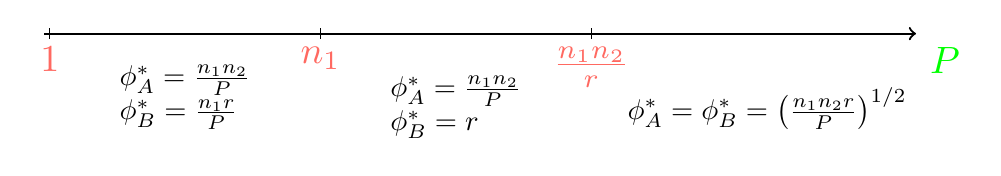
\begin{tikzpicture}[scale=0.6875, every node/.style={transform shape}]
					\draw [->, thick] (-0.1,0) -- (16,0) node [below right,pastelgreen,scale=2] {$P$};
					\draw (0, 0.1) -- node [below, pastelred, scale=2]{$1$}(0,-0.1);
					\draw (5, 0.1) -- node [below, pastelred, scale=2]{$n_1$}(5,-0.1);
					\draw (10, 0.1) -- node [below, pastelred, scale=2] {$\frac{n_1n_2}{r}$}(10,-0.1);
					
					\node[align=left,below,scale=1.5] at (2.5, -0.4) {$\phi_A^*=\frac{n_1n_2}{P}$\\ $\phi_B^*=\frac{n_1r}{P}$};
					\node[align=left,below,scale=1.5] at (7.5, -0.6) {$\phi_A^*=\frac{n_1n_2}{P}$\\ $\phi_B^*=r$};
					\node[align=center,below,scale=1.5] at (13.25, -0.8) {$\phi_A^*=\phi_B^*= \left(\frac{n_1n_2r}{P}\right)^{1/2}$};	
				\end{tikzpicture}
			\end{center}
			\vspace*{-0.25cm}
			\item Communication lower bound = $\phi_A + \phi_B - \text{data owned by the processor} = \phi_A + \phi_B - \frac{n_1n_2+n_1r}{P}$
		\end{itemize}
	\end{block}
\end{frame}
\subsection{Optimal algorithms}
\begin{frame}{Table of Contents} 
	\tableofcontents[currentsubsection] % Output the table of contents (all sections on one slide)
\end{frame}

\begin{frame}{A naive way to minimize communication cost for $B=A\Omega$}
	$$\begin{pmatrix}
	B_1\\
	B_2\\
	B_3		
	\end{pmatrix}=\begin{pmatrix}
	A_1\\
	A_2\\
	A_3		
	\end{pmatrix}\cdot \Omega$$
	\vfill
	Structure of the algorithm for each processor $i$:
	\begin{itemize}
		\item owns $A_i$ row block ($1/P$ th portion of $A$), generates random matrix $\Omega$, and \\performs $B_i = A_i \cdot \Omega$ 
	\end{itemize}
	\vfill
	When $P$ is small, communication cost of the algorithm is $0$ (\alert{Optimal}).
	
		\vfill
	\begin{center}	
		\alert{What about when $P$ is large?}
	\end{center}
	
	\vfill
\end{frame}

\begin{frame}{Matrix multiplication with a random matrix}
	\vspace*{-0.15cm}
	\begin{algorithmic}[1]		
		\Require $\Pi$ is a $p_1\times p_2 \times p_3$  grid of processors, $|\Pi| = P$.
		\Require $\M{A}$ is evenly divided into a $p_1\times p_2$ grid of rectangular blocks of dimension $n_1/p_1\times n_2/p_2$, and each block $\M{A}_{ij}$ is evenly divided across a set of $p_3$ processors. $\M{A}_{ij}^{(k)}$ is owned by processor rank $(i,j,k)$.
		\Ensure $\M{B} = \M{A}\M{\Omega}$, $\M{B}$ is evenly divided across a $p_1\times p_3$ grid of blocks, and each block $\M{B}_{ik}$ is evenly divided across a set of $p_2$ processors. $\M{B}_{ik}^{(j)}$ is owned by processor rank $(i,j,k)$.
		\Function{$\M{B}_{ik}^{(j)}=$ RandMatMul}{$\M{A}_{ij}^{(k)},\Pi$}
		\State $(i,j,k) = \Call{MyRank}{\Pi}$
%		\State //Gather the required data of input matrix $\M{A}$
		\State $\M{A}_{ij}$ = \Call{All-Gather}{$\M{A}_{ij}^{(k)}$, $\Pi_{ij*}$}\Comment{Gather the required data of input matrix $\M{A}$}
%		\State //Generate the required random submatrix
		\State $\M{\Omega}_{jk}$ =  \Call{GenRandom}{$n_2/p_2,r/p_3$} \Comment{Generate the required random submatrix}
		%		\State $\M{\Omega}_{jk}$ =  \Call{Random}{$(n_2/p_2,r/p_3)$,seed$=j(r/p_3)+k$}
%		\State //Perform local matrix multiplication
		\State $\bar{\M{B}_{ik}}=\M{A}_{ij} \cdot \M{\Omega}_{jk}$\Comment{Perform local matrix multiplication}
%		\State //Sum results to compute $\M{B}_{ik}^{(j)}$
		\State $\M{B}_{ik}^{(j)} = \Call{Reduce-Scatter}{\bar{\M{B}_{ik}},\Pi_{i*k}}$\Comment{Sum results to compute $\M{B}_{ik}^{(j)}$}
		\EndFunction
	\end{algorithmic}

	\vfill
 \brown{Communication cost is optimal when $p_1$, $p_2$ \& $p_3$ are chosen based on lower bounds.}

	\vfill
\end{frame}

\section{Computations of Nyström approximation}
\subsection{$A\Omega$ and $\Omega^TA\Omega$ computations together}

\begin{frame}{Table of Contents} 
	\tableofcontents[currentsubsection] % Output the table of contents (all sections on one slide)
\end{frame}

\begin{frame}{Nyström approximation}
Let $\M{A} \in \mathbb{R}^{n\times n}$ be a symmetric positive definite matrix and $\M{\Omega} \in \mathbb{R}^{n\times r}$ be a random matrix.

	\begin{itemize}
		\item Nyström approximation of $\M{A}$, $\widetilde{\M{A}} = (\M{A}\M{\Omega}) (\M{\Omega}^T\M{A}\M{\Omega})^\dag (\M{A}\M{\Omega})^T$ 
		\item Requires to compute both $\M{A}\M{\Omega}$ and $\M{\Omega}^T\M{A}\M{\Omega}$
	\end{itemize}


	\begin{block}{Constraints for load balanced computation}
		\centering$\M{B}=\M{A}\M{\Omega}, \quad \M{C}=\M{\Omega}^T\M{B}$
		\begin{itemize}
			\item $\phi_A, \phi_B, \phi_C$ : projections of computations on arrays $A$, $B$, $C$
			\item Each processor performs $1/P$th portion of each computation
			\item From the HBL inequality: $\phi_A \phi_B  \geq \frac{n^2r}{P}$, $\phi_B \phi_C  \geq \frac{nr^2}{P}$
			\item Extra constraints: $\frac{n^2}{P} \leq \phi_A \leq n^2$, $\frac{nr}{P} \leq \phi_B \leq nr$, $\frac{r^2}{P}\leq \phi_C\leq r^2$
		\end{itemize}
		\hfill
	\end{block}
\end{frame}
\begin{frame}{Optimization problem and communication lower bounds}
	\footnotesize
	\begin{center}
		\vspace*{-0.375cm}\begin{align*}
		Minimize &\ \phi_A + \phi_B  +\phi_C  \text{ s.t.}\\
		\phi_A \phi_B \geq \frac{n^2r}{P} & \phi_B \phi_C \geq \frac{nr^2}{P}\\
		\frac{n^2}{P} \leq \phi_A \leq n^2, \frac{nr}{P} & \leq \phi_B \leq nr, \frac{r^2}{P}\leq \phi_C\leq r^2
		\end{align*}
	\end{center}
	\vspace*{-0.25cm}
	\begin{block}{Amount of non-random array accesses = $\phi_A + \phi_B + \phi_C$}
		\begin{itemize}\small
			\item Estimate the solution and prove optimality using all Karush--Kuhn--Tucker conditions are satisfied
			\item For $n\geq r$,
				\begin{center}
				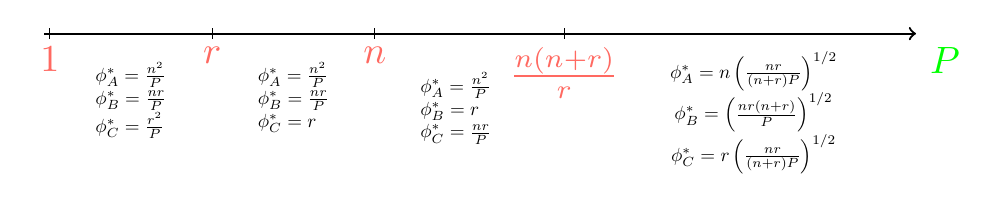
\begin{tikzpicture}[scale=0.6875, every node/.style={transform shape}]
				\draw [->, thick] (-0.1,0) -- (16,0) node [below right,pastelgreen,scale=2] {$P$};
				\draw (0, 0.1) -- node [below, pastelred, scale=2]{$1$}(0,-0.1);
				\draw (3, 0.1) -- node [below, pastelred, scale=2]{$r$}(3,-0.1);
				\draw (6, 0.1) -- node [below, pastelred, scale=2] {$n$}(6,-0.1);
				\draw (9.5, 0.1) -- node [below, pastelred, scale=2] {$\frac{n(n+r)}{r}$}(9.5,-0.1);
				
				\node[align=left,below,scale=1.0] at (1.5, -0.4) {$\phi_A^*=\frac{n^2}{P}$\\ $\phi_B^*=\frac{nr}{P}$\\ $\phi_C^*=\frac{r^2}{P}$};
				\node[align=left,below,scale=1.0] at (4.5, -0.4) {$\phi_A^*=\frac{n^2}{P}$\\ $\phi_B^*=\frac{nr}{P}$\\ $\phi_C^*=r$};		\node[align=left,below,scale=1.0] at (7.5, -0.6) {$\phi_A^*=\frac{n^2}{P}$\\ $\phi_B^*=r$\\ $\phi_C^*=\frac{nr}{P}$};
				\node[align=center,below,scale=1.0] at (13, -0.2) {$\phi_A^*=n\left(\frac{nr}{(n+r)P}\right)^{1/2}$\\ $\phi_B^*=\left(\frac{nr(n+r)}{P}\right)^{1/2}$\\ $\phi_C^*= r\left(\frac{nr}{(n+r)P}\right)^{1/2}$};	
				\end{tikzpicture}
			\end{center}
			\vspace*{-0.25cm}
			\item Communication lower bound = $\phi_A + \phi_B + \phi_C - \text{data owned by the processor}$\\  $\qquad\qquad\qquad\qquad\qquad\qquad=\phi_A + \phi_B + \phi_C - \frac{n^2+nr+r^2}{P}$
		\end{itemize}
	\end{block}
\end{frame}
\subsection{Optimal algorithms}
\begin{frame}{Table of Contents} 
	\tableofcontents[currentsubsection] % Output the table of contents (all sections on one slide)
\end{frame}


\begin{frame}{Parallel algorithms for $\M{B}=\M{A}\M{\Omega}$ and $\M{C}=\M{\Omega^T}\M{B}$}
	\vspace*{-0.15cm}
	\small
	\begin{algorithmic}[1]
		\Require $\Pi$ is a $p_1\times p_2 \times p_3$  processor grid, $\Psi$ is a $q_1 \times q_2 \times q_3$ processor grid, and $|\Pi| = |\Psi| = P$.
		\Require $\M{A}$ is evenly divided into a $p_1\times p_2$ grid of rectangular blocks, and each block $\M{A}_{ij}$ is evenly divided across a set of $p_3$ processors with $\M{A}_{ij}^{(k)}$ is owned by processor rank $(i,j,k)$ in $\Pi$.
		\Ensure $\M{B} = \M{A}\M{\Omega}$, $\M{B}$ is evenly divided across a $q_1\times q_3$ grid of blocks, and each block $\M{B}_{i'k'}$ is evenly divided across a set of $q_2$ processors with $\M{B}_{i'k'}^{(j')}$ is owned by processor rank $(i',j',k')$ in $\Psi$.
		\Ensure $\M{C} = \M{\Omega^T}\M{B}$, $\M{C}$ is evenly divided across a $q_2\times q_3$ grid of blocks, and each block $\M{C}_{j'k'}$ is evenly divided across a set of $q_1$ processors with $\M{C}_{j'k'}^{(i')}$ is owned by processor rank $(i',j',k')$ in $\Psi$.
		\Function{$(\M{B}_{i'k'}^{(j')},\M{C}_{j'k'}^{(i')})=$ RandCompNys}{$\M{A}_{ij}^{(k)},\Pi, \Psi$}
		\State $(i,j,k) = \Call{MyRank}{\Pi}$
		\State Perform $\M{B} = \M{A}\M{\Omega}$ in $p_1\times p_2 \times p_3$  grid of processors
		\State //Change distribution of $\M{B}$ so that it is suitable for $q_1 \times q_2 \times q_3$ grid 
		\State $(i',j',k') = \Call{MyRank}{\Psi}$
%		\If{\textbf{if} \emph{for any} $i, p_i \neq q_i$ \textbf{then}}
		\State {\textbf{if} \emph{for any} $i, p_i \neq q_i$ \textbf{then}} $\M{B}_{i'k'}^{(j')} $ = \Call{Redistribute}{$\M{B}$} {\textbf{end if}}
%		\EndIf
		\State Perform $\M{C}=\M{\Omega^T}\M{B}$ in $q_1\times q_2 \times q_3$  grid of processors
		\EndFunction
		\end{algorithmic}
\end{frame}

\begin{frame}{Processor grid dimensions}
	\begin{itemize}
		\item Not clear how to obtain processor grid dimensions that exactly match lower bounds ($p_i=q_i$ for $i=0,1,2$)
	\end{itemize}
\vfill
Approach 1 (\brown{\emph{Redist}ribution}):
\begin{itemize}
	\item Perform $\M{B} = \M{A}\M{\Omega}$ in $p_1\times p_2 \times p_3$ grid of processors and $\M{C}=\M{\Omega^T}\M{B}$ in $q_1\times q_2 \times q_3$  grid of processors
	\begin{itemize}
		\item Communication cost is far from the lower bound by the sum of the communication cost of $B$ and the redistribution cost 
	\end{itemize} 
\end{itemize}
\vfill
Approach 2 (\brown{\emph{No-Redist}ribution}):
\begin{itemize}
	\item $\M{B} = \M{A}\M{\Omega}$ is the dominating computation
	\begin{itemize}
		\item Use the optimal processor grid of this computation to also perform $\M{C}=\M{\Omega^T}\M{B}$
	\end{itemize}
\end{itemize}
\vfill
\end{frame}

\begin{frame}{\emph{Redist}ribution  vs \emph{No-Redist}ribution on $3$ processors}
		\centering
	%!TEX root = ../paper.tex
\newcommand{\nOne}{9}
\newcommand{\nTwo}{9}
\newcommand{\nThree}{3}
\newcommand{\nP}{3}
\pgfmathsetmacro{\offset}{.33}
\newcommand{\mycolor}{red}
\newcommand{\x}{0}

\newcommand{\shadingleft}{
% top face of left comp cube
\begin{scope}[canvas is zx plane at y=(\nTwo-.5-\x),rotate=90,shift={(-\nOne+.5,-.5)}]
	\draw[draw=\mycolor,fill=\mycolor!25] (0,\nThree) rectangle (\nOne,0);
\end{scope}
% right face of left comp cube
\begin{scope}[canvas is yz plane at x=.5,rotate=-90,yscale=-1,shift={(-.5,-\nOne+.5+\x)}]
	\draw[draw=\mycolor,fill=\mycolor!25] (0,0) rectangle (\nThree,\nOne/\nP);
\end{scope}
%front face of left comp cube
\begin{scope}[canvas is yx plane at z=.5,yscale=-1,rotate=180,shift={(-\nTwo+\x+.5,.5)}]
	\draw[draw=\mycolor,fill=\mycolor!25] (0,0) rectangle (\nOne/\nP,-\nOne);
\end{scope}
}

\newcommand{\shadingright}{
%front face of right comp cube
\begin{scope}[canvas is yx plane at z=.5-\x,yscale=-1,rotate=180,shift={(.5,.5)}]
	\draw[draw=\mycolor,fill=\mycolor!25] (0,0) rectangle (-\nOne,\nThree);
\end{scope}
% right face of right comp cube
\begin{scope}[canvas is yz plane at x=.5+\nThree,rotate=-90,yscale=-1,shift={(-.5+\x,-\nOne+.5)}]
	\draw[draw=\mycolor,fill=\mycolor!25] (0,0) rectangle (\nThree/\nP,\nOne);
\end{scope}
% top face of right comp cube
\begin{scope}[canvas is zx plane at y=(\nTwo-.5),rotate=90,shift={(.5,-.5+\x)}]
	\draw[draw=\mycolor,fill=\mycolor!25] (0,0) rectangle (\nThree,\nThree/\nP);
\end{scope}
}

\newcommand{\shadingnoredist}{
%front face
\begin{scope}[canvas is yx plane at z=.5,yscale=-1,rotate=180,shift={(-\nTwo+\x+.5,.5)}]
	\draw[draw=\mycolor,fill=\mycolor!25] (0,\nThree) rectangle (\nOne/\nP,-\nOne);
\end{scope}
% top face 
\begin{scope}[canvas is zx plane at y=(\nTwo-.5-\x),rotate=90,shift={(-\nOne+.5,-.5)}]
	\draw[draw=\mycolor,fill=\mycolor!25] (0,\nThree) rectangle (\nOne+\nThree,0);
\end{scope}
% right face 
\begin{scope}[canvas is yz plane at x=.5+\nThree,rotate=-90,yscale=-1,shift={(-.5,-\nOne+.5+\x)}]
	\draw[draw=\mycolor,fill=\mycolor!25] (0,0) rectangle (\nThree,\nOne/\nP);
\end{scope}
}

\newcommand{\compprism}{
% dimension labels
\node[shift={(.5,-.5,.5)},scale=2] at (-\nOne/2,-0.5,0) {$n$};
\node[shift={(.5,-.5,.5)},scale=2] at (\nThree/2,-0.5,0) {$r$};
\node[shift={(.5,-.5,.5)},scale=2] at (\nThree+0.5/2,-0.5/2,-\nThree/2) {$r$};
\node[shift={(.5,-.5,.5)},scale=2] at (-\nOne-0.5,\nTwo/2,0) {$n$};

% right face of comp cube
\begin{scope}[canvas is yz plane at x=.5,rotate=-90,yscale=-1,shift={(-.5,-\nTwo+.5)}]
	\draw[black,xscale=\nThree/1,yscale=\nTwo/1] (0,0) grid (1,1);
	\node[yscale=-1,scale=2] at (\nThree/2,\nTwo/2) {\Huge$\M{B}$};
\end{scope}
		
% left face of comp cube
\begin{scope}[canvas is yz plane at x=.5-\nOne,rotate=-90,yscale=-1,shift={(-.5,-\nTwo+.5)}]
	\draw[black,dashed,xscale=\nThree/1,yscale=\nTwo/1] (0,0) grid (1,1);
\end{scope}

% front face of comp cube
\begin{scope}[canvas is yx plane at z=.5,yscale=-1,rotate=180,shift={(-\nTwo+.5,-\nOne+.5)}]
	\draw[black,xscale=\nTwo/1,yscale=\nOne/1] (0,0) grid (1,1);
	\node[rotate=90,scale=2] at (\nTwo/2,\nOne/2) {\Huge$\M{A}$};
\end{scope}

% back face of comp cube
\begin{scope}[canvas is yx plane at z=.5-\nThree,yscale=-1,rotate=180,shift={(-\nTwo+.5,-\nOne+.5)}]
	\draw[black,dashed,xscale=\nTwo/1,yscale=\nOne/1] (0,0) grid (1,1);
\end{scope}

% top face of left comp cube
\begin{scope}[canvas is zx plane at y=(\nTwo-.5),rotate=90,shift={(-\nOne+.5,-.5)}]
	\draw[black,xscale=\nOne/1,yscale=\nThree/1] (0,0) grid (1,1);
	\node[rotate=90,scale=2] at (\nOne/2,\nThree/2) {\Huge$\M{\Omega}$};
\end{scope}
		
% top face of right comp cube
\begin{scope}[canvas is zx plane at y=(\nTwo-.5),rotate=90,shift={(.5,-.5)}]
	\draw[black,xscale=\nThree/1,yscale=\nThree/1] (0,0) grid (1,1);
	\node[rotate=90,scale=2] at (\nThree/2,\nThree/2) {\Huge$\M{C}$};
\end{scope}
		
% front face of right comp cube
\begin{scope}[canvas is yx plane at z=.5,yscale=-1,rotate=180,shift={(.5,.5)}]
	\draw[black,xscale=\nTwo/1,yscale=\nThree/1] (0,0) grid (-1,1);
	\node[rotate=90,scale=2] at (-\nTwo/2,\nThree/2) {\Huge$\M{\Omega}$};
\end{scope}
		
% right face of right comp cube
\begin{scope}[canvas is yz plane at x=.5+\nThree,rotate=-90,yscale=-1,shift={(-.5,-\nTwo+.5)}]
	\draw[black,xscale=\nThree/1,yscale=\nTwo/1] (0,0) grid (1,1);
	\node[yscale=-1,scale=2] at (\nThree/2,\nTwo/2) {\Huge$\M{B}$};
\end{scope}
		
% back face of rightcomp cube
\begin{scope}[canvas is yx plane at z=.5-\nThree,yscale=-1,rotate=180,shift={(-\nTwo+.5,.5)}]
	\draw[black,dashed,xscale=\nTwo/1,yscale=\nThree/1] (0,0) grid (1,1);
\end{scope}
}



\begin{tikzpicture}[every node/.append style={transform shape},scale=.45]
		
	% shade processor assignments for 1d-redist-1d 1st matmul	
	\renewcommand{\x}{6}
	\renewcommand{\mycolor}{blue}
	\shadingleft
		
	\renewcommand{\x}{3}
	\renewcommand{\mycolor}{green}
	\shadingleft
			
	\renewcommand{\x}{0}
	\renewcommand{\mycolor}{red}
	\shadingleft	
			
	% shade processor assignments for 1d-redist-1d 2nd matmul	
	\renewcommand{\x}{2}
	\renewcommand{\mycolor}{blue}
	\shadingright
			
	\renewcommand{\x}{1}
	\renewcommand{\mycolor}{green}
	\shadingright
			
	\renewcommand{\x}{0}
	\renewcommand{\mycolor}{red}
	\shadingright
		
	% draw computational prism structure
	\compprism
	
	\begin{scope}[shift={(\nOne+\nThree+\nThree,0)}]
		% shade processor assignments for 1d-redist-1d 1st matmul	
		\renewcommand{\x}{6}
		\renewcommand{\mycolor}{blue}
		\shadingnoredist
		
		\renewcommand{\x}{3}
		\renewcommand{\mycolor}{green}
		\shadingnoredist
			
		\renewcommand{\x}{0}
		\renewcommand{\mycolor}{red}
		\shadingnoredist
	
		% draw computational prism structure
		\compprism
	\end{scope}

\end{tikzpicture}



\vfill	
	Total number of iteration points = $n^2r + nr^2=n(n+r)r$
\vfill
\end{frame}

\section{Experimental results}
\begin{frame}{Table of Contents} 
	\tableofcontents[currentsection] % Output the table of contents (all sections on one slide)
\end{frame}

\begin{frame}{Experimental settings}
	\begin{center}

	    \begin{tabular}{r l l}
			\toprule
			\multicolumn{3}{c}{\textbf{NERSC Perlmutter GPU Partition}} \\
			\toprule
			Processor & \multicolumn{2}{c}{1 $\times$ AMD EPYC 7763 per node} \\
			\# NUMA domains & \multicolumn{2}{c}{4} \\
			\# Cores & \multicolumn{2}{c}{64 per node, 16 per NUMA domain }\\
			\# Hyperthreads & \multicolumn{2}{c}{2 per core, 32 per NUMA domain }\\
			\# GPUs & \multicolumn{2}{c}{4 $\times$ NVIDIA A100 per node }\\
			Memory & \multicolumn{2}{c}{256 GB DDR4 per node, 40GB per GPU }\\
			\toprule
			& \textbf{CPU-only} & \textbf{GPU} \\
			\toprule
			Compiler & Intel C++  & NVIDIA CUDA C++ \\
			& version 2024.1.0 & version 24.5-1 \\
			BLAS and PRNG & MKL 2024.1 & CUDA toolkit 12.4 \\
			MPI & \multicolumn{2}{c}{CRAY MPICH 8.1.30 (CUDA-aware for GPUs)} \\
			%\toprule
			\bottomrule
		\end{tabular}
	\end{center}
\end{frame}

\begin{frame}{Dataset and number of processors}
	\begin{itemize}
		\item Small number of processors ($P < r$, practical regime)
		\begin{itemize}
			\item For $\M{B} = \M{A}\M{\Omega}$ computation, communication cost = $0$
			\item For $\M{B} = \M{A}\M{\Omega}$ and $\M{C}=\M{\Omega^T}\M{B}$ computations, communication cost = $nr/P$ (for \emph{Redist}ribution) and $r^2-r^2/P$ (for \emph{No-Redist}ribution)
		\end{itemize}
		\vfill
		\item $n$ and $r$ are selected based on CIFAR-10 dataset
		\begin{itemize}
			\item $n=50,000$ and $r=500$ and $5000$ 
		\end{itemize}
	\end{itemize}
\end{frame}

\begin{frame}{C++ vs Python: 3D-distributed memory matrix multiplication}
	\begin{center}
 		 % MatMul on CPU
% Rank = 50000
% CPP vs Python

% Data file (inline table with fake values)
\pgfplotstableread[col sep=comma]{plots/data/cpp_python.csv}\datafile

\begin{tikzpicture}
\begin{axis}[\cppVSpython
    %width=0.6\linewidth,
    height=0.25\textwidth,
    after end axis/.code={ % draw after axis so it doesn't get clipped
      \node(A14) at (axis cs:Algo-\impla-\proca,0) {};
      \node(A24) at (axis cs:Algo-\implb-\proca,0) {};
      \node(A18) at (axis cs:Algo-\impla-\procb,0) {};
      \node(A28) at (axis cs:Algo-\implb-\procb,0) {};
      \node(A116) at (axis cs:Algo-\impla-\procc,0) {};
      \node(A216) at (axis cs:Algo-\implb-\procc,0) {};
      \node(A132) at (axis cs:Algo-\impla-\procd,0) {};
      \node(A232) at (axis cs:Algo-\implb-\procd,0) {};
      \node(A164) at (axis cs:Algo-\impla-\proce,0) {};
      \node(A264) at (axis cs:Algo-\implb-\proce,0) {};
      \node(A1128) at (axis cs:Algo-\impla-\procf,0) {};
      \node(A2128) at (axis cs:Algo-\implb-\procf,0) {};
      \node[yshift=-30, xshift=-5] at (A24) {\scriptsize $4$};
      \node[yshift=-30, xshift=-5] at (A28) {\scriptsize $8$};
      \node[yshift=-30, xshift=-5] at (A216) {\scriptsize $16$};
      \node[yshift=-30, xshift=-5] at (A232) {\scriptsize $32$};
      \node[yshift=-30, xshift=-5] at (A264) {\scriptsize $64$};
      \node[yshift=-30, xshift=-5] at (A2128) {\scriptsize $128$};
      % \node[anchor=south] at (axis cs:old-\mb-\pga,151) {$\vdots$};
    },
    x tick label style={font=\scriptsize},
    y tick label style={font=\scriptsize,/pgf/number format/fixed,/pgf/number format/precision=2},
    ymajorgrids
    ]
    \pgfplotsset{cycle list={black, fill=color7 \\ black, fill=color2 \\ black, fill=color1 \\ black, fill=color4 \\}}
    
    \addplot table[x=alg, y expr=(\thisrow{gatherATime})] {\datafile};
    \addplot table[x=alg, y expr=(\thisrow{gatherBTime})] {\datafile};
    \addplot table[x=alg, y expr=(\thisrow{localMultiplyTime})] {\datafile};
    \addplot table[x=alg, y expr=(\thisrow{scatterReduceTime})] {\datafile};
    \iflegend
    	\legend{Gather A, Gather B, Local Multiply, Reduce Scatter};
    \fi
  \end{axis}
\end{tikzpicture}



% alg,gatherATime,genBTime,gatherBTime,localMultiplyTime,cpuGpuDataMoveTime,scatterReduceTime

	\end{center}
\vfill
\begin{itemize}
	\item Comparison to multiply two $50k \times 50k$ double precision matrices
	\item Use a  processor grid as cubical as possible
	\item Python (mpi4py version 3.1.5) performance is hard to explain
	\item We focus on C++ implementation
\end{itemize}
\vfill
\end{frame}

\begin{frame}{Communicating vs redundantly generating $\M{\Omega}$ in $\M{B}=\M{A}\M{\Omega}$}
	
	\begin{columns}
		\begin{column}{0.24\linewidth}
			\input{plots/matmul_cpu_500.tex}
			$\qquad\qquad\qquad r = 500$
		\end{column}
		\begin{column}{0.24\linewidth}
			\input{plots/matmul_cpu_5000.tex}
			$\qquad\qquad r = 5000$
		\end{column}\hfill
	\end{columns}

\medskip
\begin{itemize}
	\item Generating $\M{\Omega}$ is cheaper than communicating it
\end{itemize}
\end{frame}

\begin{frame}{$\M{B} = \M{A}\M{\Omega}$ and $\M{C}=\M{\Omega^T}\M{B}$ computations}
	
		\begin{columns}
		\begin{column}{0.24\linewidth}
			
\begin{tikzpicture}
    \begin{axis}[
        xlabel={P},
        ylabel={Time (seconds)},
        ymin=0,         grid=major,
        xmode=log,
	log basis x=2,
	ymode=log,
	log basis y=2,
	width=4.8cm, height=4.5cm,
	legend style={
        at={(0.25,1.15)},     % Position (x,y)
        anchor=west,         % Anchor point of legend box
    },
     legend columns=2,
      legend style={draw=none, cells={align=left}, nodes={scale=0.7}},
        xtick={2^2,2^3,2^4,2^5,2^6,2^7},
        ytick={2^-3,2^-2,2^-1, 2^0, 2^1},
    ]
        \pgfplotsset{cycle list={black, fill=color1 \\ black, fill=color2 \\ black, fill=color3 \\ black, fill=color4 \\ black, fill=color5 \\ black, fill=color9 \\}}
    % Plot 1: 1DredCPU
    \addplot[
        mark=square,
        color=color1,
        thick,
    ] table [x=proc, y=1DredCPU, col sep=comma] {plots/data/lineplot500.csv};
    \addlegendentry{Redist-CPU}
    
    % Plot 2: 1DnoredCPU
    \addplot[
        mark=*,
        color=color2,
        thick,
    ] table [x=proc, y=1DnoredCPU, col sep=comma] {plots/data/lineplot500.csv};
    \addlegendentry{No-Redist-CPU}
    
    % Plot 3: 1DredGPU
    \addplot[
        mark=triangle,
        color=color3,
        thick,
    ] table [x=proc, y=1DredGPU, col sep=comma] {plots/data/lineplot500.csv};
    \addlegendentry{Redist-GPU}
    
    % Plot 4: 1DnoredGPU
    \addplot[
        mark=x,
        color=color4,
        thick,
    ] table [x=proc, y=1DnoredGPU, col sep=comma] {plots/data/lineplot500.csv};
    \addlegendentry{No-Redist-GPU}
    
    \end{axis}
\end{tikzpicture}


			$\qquad\qquad\qquad r = 500$
		\end{column}
		\begin{column}{0.24\linewidth}
			\vspace*{0.56cm}
			
			\begin{tikzpicture}
    \begin{axis}[
        xlabel={P},
        %ylabel={Time (seconds)},
        ymin=0,
        grid=major,
        xmode=log,
	log basis x=2,
	ymode=log,
	log basis y=2,
	width=4.8cm, height=4.5cm,
	 legend pos={north west},
  	legend columns=2,
  	legend style={draw=none, cells={align=left}, nodes={scale=0.7}},
        xtick={2^2,2^3,2^4,2^5,2^6,2^7},
        ytick={2^-2,2^-1,2^-0, 2^1, 2^2, 2^3, 2^4},
   ]
   
    
    % Plot 1: 1DredCPU
    \addplot[
        mark=square,
        color=color1,
        thick,
    ] table [x=proc, y=1DredCPU, col sep=comma] {plots/data/lineplot5000.csv};
    
    
    % Plot 2: 1DnoredCPU
    \addplot[
        mark=*,
        color=color2,
        thick,
    ] table [x=proc, y=1DnoredCPU, col sep=comma] {plots/data/lineplot5000.csv};
    
    % Plot 3: 1DredGPU
    \addplot[
        mark=triangle,
        color=color3,
        thick,
    ] table [x=proc, y=1DredGPU, col sep=comma] {plots/data/lineplot5000.csv};
    
    % Plot 4: 1DnoredGPU
    \addplot[
        mark=x,
        color=color4,
        thick,
    ] table [x=proc, y=1DnoredGPU, col sep=comma] {plots/data/lineplot5000.csv};
    
    \end{axis}
\end{tikzpicture}

			$\qquad\qquad r = 5000$
		\end{column}\hfill
	\end{columns}
	
	\medskip
	\begin{itemize}
		\item CPU-only implementations scale better
		\item \emph{Redist} approach scales better on GPU
	\end{itemize}

\end{frame}
\begin{frame}{Runtime breakdown for both approaches with $r=5000$}
	\vspace*{-0.15cm}
			\begin{columns}
		\begin{column}{0.21\linewidth}
			% Nystrom on CPU
% Rank = 5000

% Data file (inline table with fake values)
\pgfplotstableread[col sep=comma]{plots/data/nystrom_cpu_5000.csv}\datafile


\begin{tikzpicture}
 \begin{axis}[\nystromCPUrankFiveTall
    after end axis/.code={ % draw after axis so it doesn't get clipped
      \node(A14) at (axis cs:Algo-\algoa-\proca,0) {};
      \node(A24) at (axis cs:Algo-\algob-\proca,0) {};
      \node(A18) at (axis cs:Algo-\algoa-\procb,0) {};
      \node(A28) at (axis cs:Algo-\algob-\procb,0) {};
      \node(A116) at (axis cs:Algo-\algoa-\procc,0) {};
      \node(A216) at (axis cs:Algo-\algob-\procc,0) {};
      \node(A132) at (axis cs:Algo-\algoa-\procd,0) {};
      \node(A232) at (axis cs:Algo-\algob-\procd,0) {};
      \node(A164) at (axis cs:Algo-\algoa-\proce,0) {};
      \node(A264) at (axis cs:Algo-\algob-\proce,0) {};
      \node(A1128) at (axis cs:Algo-\algoa-\procf,0) {};
      \node(A2128) at (axis cs:Algo-\algob-\procf,0) {};
      \node[yshift=-35, xshift=-5] at (A24) {\scriptsize $4$};
      \node[yshift=-35, xshift=-5] at (A28) {\scriptsize $8$};
      \node[yshift=-35, xshift=-5] at (A216) {\scriptsize $16$};
      \node[yshift=-35, xshift=-5] at (A232) {\scriptsize $32$};
      \node[yshift=-35, xshift=-5] at (A264) {\scriptsize $64$};
      \node[yshift=-35, xshift=-5] at (A2128) {\scriptsize $128$};
      % \node[anchor=south] at (axis cs:old-\mb-\pga,151) {$\vdots$};
    },
    x tick label style={font=\scriptsize},
    y tick label style={font=\scriptsize,/pgf/number format/fixed,/pgf/number format/precision=2},
        grid=both,
    major grid style={line width=0.8pt, draw=gray!50},
     minor grid style={line width=0.4pt, draw=gray!20},
    minor tick num=5
    ]
    \pgfplotsset{cycle list={black, fill=color3 \\ black, fill=color1 \\ black, fill=color5 \\ black, fill=color9 \\ black, fill=color8 \\ black, fill=color4 \\}}
    
    \addplot table[x=alg, y expr=(\thisrow{genOmegaTime})] {\datafile};
     \addplot table[x=alg, y expr=(\thisrow{dgemm1Time})] {\datafile};
    \addplot table[x=alg, y expr=(\thisrow{all2allTime})] {\datafile};
    \addplot table[x=alg, y expr=(\thisrow{unpackTime})] {\datafile};
     \addplot table[x=alg, y expr=(\thisrow{dgemm2Time})] {\datafile};
      \addplot table[x=alg, y expr=(\thisrow{reduceScatterTime})] {\datafile};
    
    \iflegend
    	\legend{Generate B,  1st MatMul , All2All, Unpack, 2nd MatMul, ReduceScatter};
    \fi
  \end{axis}
\end{tikzpicture}

%alg,totalTime,genOmegaTime,dgemm1Time,dgemm2Time,all2allTime,reduceScatterTime,reduceScatter1Time,reduceScatter2Time,unpackTime,packTime

			\vspace*{-0.15cm}$\qquad\qquad\qquad\text{CPU}$
		\end{column}
		\begin{column}{0.21\linewidth}
			\vspace*{0.56cm}
			\input{plots/nystrom_gpu_5000_all.tex}
			\vspace*{-0.15cm}$\qquad\qquad\qquad\text{GPU}$
		\end{column}\hfill
	\end{columns}
\vfill
%	\vspace*{-0.15cm}
%	\medskip
	\begin{itemize}
		\item CPU-only implementation is dominated by the local matrix multiplication
	\end{itemize}
\vfill
\end{frame}

\section{Conclusion}
\begin{frame}{Table of Contents} 
	\tableofcontents[currentsection] % Output the table of contents (all sections on one slide)
\end{frame}
\begin{frame}{Conclusion and future work}
	\begin{block}{Conclusion}
		\begin{itemize}
			\item Communication lower bounds and optimal algorithms for $\M{B} = \M{A}\M{\Omega}$ and $\M{C}=\M{\Omega^T}\M{B}$
			\item Parallel scalability of our algorithms on both CPUs and GPUs
			\item \emph{Redist} approach scales better on GPUs
		\end{itemize}
	\end{block}
	\vfill
	\begin{block}{Future Work}
		\begin{itemize}
			\item Exploit symmetry to further reduce computation and communication costs
			\item Study how to perform all computations of generalized Nyström approximations for nonsymmetric matrices efficiently
			\item Extend our approaches to other sketching methods that use structured matrices, such as CountSketch and Subsampled Randomized Hadamard Transform methods
		\end{itemize}
	\end{block}
\end{frame}

%\begin{frame}{Planning}
%	\begin{itemize}
%%		\item Lower bound
%%		\item Existing results for Matrix multiplication
%%		\item Importance of $A\Omega$ computation
%%		\item Communication lower bounds and results for $A\Omega$
%%		\item $A\Omega$ and $\Omega^T A\Omega$ computations
%%		\item Practical results
%	\end{itemize}
%\end{frame}


\begin{frame}
	\Huge{\centerline{Thank You!}}
\end{frame}

\end{document}










